\documentclass[12pt, a4paper]{article}
\usepackage[utf8]{inputenc}

% Format
\usepackage{layout}
\setlength{\parindent}{0.5in}
\setcounter{secnumdepth}{0}
\usepackage{lineno}
%\usepackage{authblk}

% Font
\usepackage{MinionPro}
\input glyphtounicode
\pdfgentounicode=1
\usepackage{microtype}
\usepackage[super]{nth}

% Language
\usepackage[british]{babel}

% References
\usepackage[nosectionbib, tocbib, unnumberedbib]{apacite}

% Figures
\usepackage{graphicx}
\usepackage[small, labelfont=it, labelsep=period]{caption}

% Tables
\usepackage{booktabs}
\usepackage{tabularx}

% Commands
\newcommand{\pest}[4]{$ \text{Pr} (\text{``us''} | \text{#1}) = #2$, $[#3, #4]$}
\newcommand{\pdif}[4]{$ \Delta\text{Pr} (\text{``us''} | \text{#1}) = #2$, $[#3, #4]$}

% Frontmatter
\title{Intergroup contact fosters\\more inclusive social identities}
\date{November 5, 2018}
%\author{Nils Karl Reimer}
%\author[2]{Shanmukh V. Kamble}
%\author[3]{Katharina Schmid}
%\author[1]{Miles Hewstone}
%\affil[1]{University of Oxford}
%\affil[2]{Karnatak University}
%\affil[3]{ESEADE Business School, Ramon Llull University}
%\renewcommand\Affilfont{\small}

\begin{document}

\maketitle

\begin{abstract}
\noindent We examined how people construct their social identities from multiple group memberships---and whether intergroup contact can reduce bias by fostering more inclusive identities. Participants ($N = 351$) viewed 24 identity cards, each representing a person with whom participants shared none, one, two, or all three group memberships. Participants reported whether they considered each person as ``us'' or ``not us'', showing whom they included in their ingroup, and whom they excluded. We found that participants from diverse caste backgrounds tended to exclude caste and religious outgroups, replicating persistent social divides in South India. Bridging these divides, cross-group friendship was associated with more inclusive identities which, in turn, were associated with more favourable outgroup attitudes. Negative contact was associated with less inclusive identities, showing that past experiences shaped whom participants considered ``us'' and ``not us''. Contact and identity processes were unrelated to support for affirmative action in advantaged and disadvantaged groups.\\[1ex]
\noindent \textbf{Keywords:} intergroup contact, social identity, multiple categorization, intergroup relations, affirmative action, caste, nationalism \\[1ex]
\end{abstract}

\linenumbers

\noindent How we feel about and act toward others depends on whom we consider ``us'' and ``them''---that is, whom we include in our ingroup, and whom we exclude (for a review, see \citeNP{authors_theories_inpress}). In some situations, it is clear who is in the ingroup and who is not. On a football pitch, for example, players tend to think of their own team as ``us'', and of the other team as ``them'', and try their best to make their own team win. In diverse settings, this distinction is less clear because people belong to multiple, overlapping groups. Individuals differ in how they construct their ingroup from these group memberships. Some espouse narrow definitions of who is ``us'' and ``them'', while others adopt more inclusive identities (see Figure~\ref{fig:f1}). Many Americans, for example, associate being American with being White American \cite{devos_american_2005}. This suggests that whom Americans consider ``us'' and ``them'' might depend on someone's race \emph{and} nationality. In this paper, we examine how group memberships shape whom people consider ``us'' and ``not us'', and whether intergroup contact can reduce prejudice by fostering inclusive social identities.

\begin{figure}
\centering
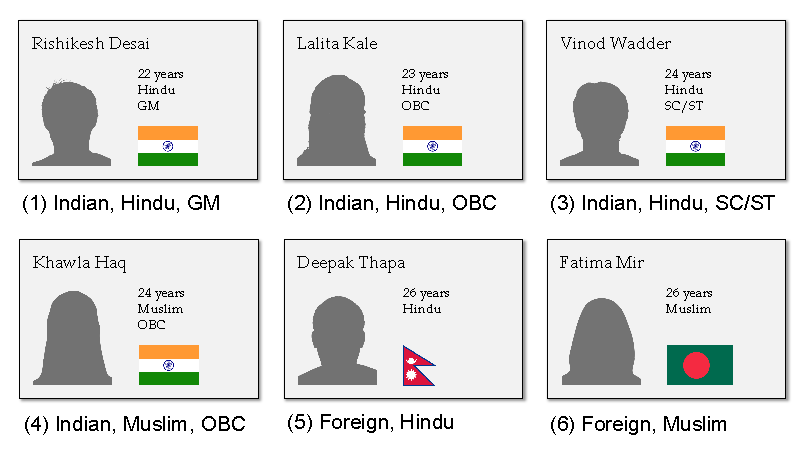
\includegraphics[scale=1]{../figures/figure-1}
\caption{
Schematic representations of social identity structures, ordered by social identity inclusiveness \protect\cite{dommelen_construing_2015}. Shaded regions represent the groups which a participant has to categorize as ``us'' to be assigned that structure. An Indian Hindu, for example, may consider only people who share their nationality, religion, and caste as ingroup members (intersection). Someone else may consider all their fellow Indians, whatever their religion or caste, as ingroup members (dominance). Another person may consider anyone who shares their nationality or religion as ingroup members (merger).
}
\label{fig:f1}
\end{figure}

\nolinenumbers

\bibliographystyle{apacite}
\bibliography{references}

\end{document}